% !TeX encoding = UTF-8
%


% Besserer Vorschlag: 
% Screenshot von ReportGenerator
% sieht schöner aus ...
% zum Schluss machen und einfach als Bild
% einfügen!

% TODO: Seitennummern!



\subsection{Abdeckung}
\label{Abschnitt:Tests:Statistik:Abdeckung}

% Coverage, welche unser lokales Werkzeug ausgibt.
\newcommand\VSLocalCoverage{\textasciitilde~84 ??? \%}

% Coverage, welche unser Online-Wekrzeug ausgibt.
\newcommand\OnlineLocalCoverage{\textasciitilde~87 ??? \%}

% Coverage im Bezug auf alle vorhandenen Klassen.
\newcommand\VSGlobalCoverage{\textasciitilde~30 \%}

Auf den folgenden Seiten steht die Kurzversion des aus den Daten von OpenCover generierten Berichts zur Testabdeckung durch Komponententests.
Der prozentuale Anteil bezieht sich hierbei auf die Anzahl der abgedeckten Zeilen Code (LOC), aller als relevant eingestufter Komponenten. In Tabelle \ref{Abschnitt:Tests:Statistik:Abdeckung:Tabelle} sind die Ergebnisse aufgelistet.

\begin{longtable}{p{0.5\hsize}p{0.5\hsize}}

	\caption{Testabdeckung durch Komponententests\\~\\}
	\label{Abschnitt:Tests:Statistik:Abdeckung:Tabelle}
	\\

	  Selektiv, lokal:
	& \VSLocalCoverage \\
	
	  Selektiv, online:
	& \OnlineLocalCoverage \\
	
	  Gesamt:
	& \VSGlobalCoverage \\

\end{longtable}

~\\

Die selektive Testabdeckung bezieht sich auf den Anteil aller Klassen die wir nicht herausgefiltert haben. Dabei verwendeten wir ein lokales- und ein Online-Werkzeug. Beide basieren auf OpenCover. Online läuft die aktuellste Version von OpenCover. Lokal erreichen wir eine Abdeckung von \VSLocalCoverage~und online \OnlineLocalCoverage. Der Unterschied kommt hauptsächlich durch die unterschiedlichen Versionen von OpenCover und kleinere Abweichungen in der Aktualität zustande. Wir geben hier beide Werte an, da diese für uns auch laufend eine Selbstkontrolle darstellen. Die Gesamt-Testabdeckung ist um einiges niedriger als die selektiven Testabdeckungen. Dies liegt daran, dass wir z.B. alle GUI-Klassen selbst geschrieben haben (Widgets, etc.). Wir verweisen an dieser Stelle nochmals auf die ausführliche Erklärung unter Abschnitt \hyperref[Abschnitt:Tests:Nicht]{\mousecursor~\ref{Abschnitt:Tests:Nicht}, ab S. \pageref{Abschnitt:Tests:Nicht}}.


%\newgeometry{left=8cm,bottom=0.1cm,top=1cm,right=0.1cm}
\newgeometry{includehead,includefoot,
  left=1.in,right=1.0in,
  top=0.6in,bottom=0.8in,
  headheight=20pt,headsep=0.25in,
  footskip=0.3in}

\thispagestyle{empty}
\pagestyle{empty}

\begin{figure}[h!]

	\centering{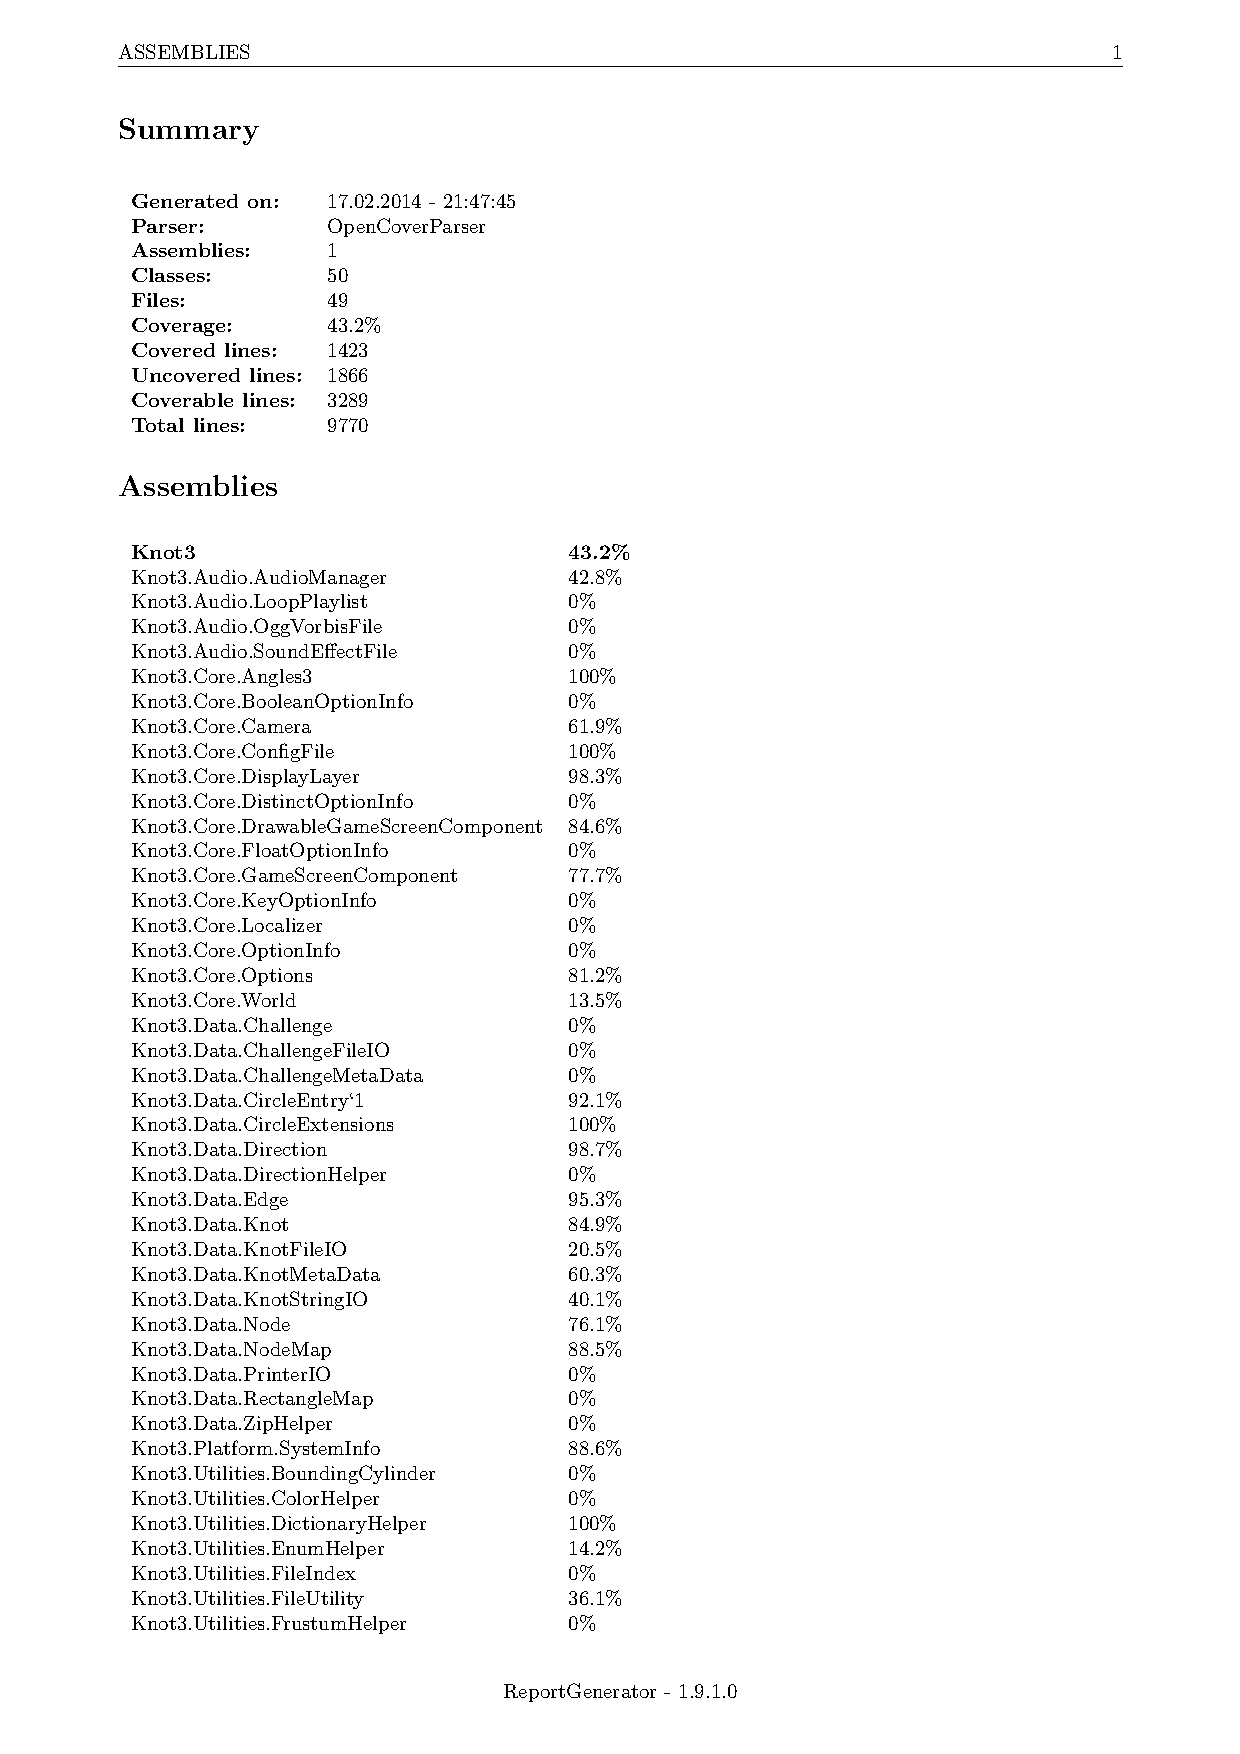
\includegraphics[page=1,scale=1.0]{Inhalt/Tests/Abdeckung/OpenCover_Bericht_uebersicht.pdf}} 
   
\end{figure}


\begin{figure}[h!]

	\centering{\includegraphics[page=2,scale=1.0]{Inhalt/Tests/Abdeckung/OpenCover_Bericht_uebersicht.pdf}} 
   
\end{figure}

\restoregeometry

\thispagestyle{plain}
\pagestyle{plain}